\documentclass{article}

\usepackage[usenames]{color} 
\usepackage{graphicx} 

\definecolor{lightblue}{rgb}{0.0, 0.8,1.0} 
\definecolor{myOrange}{rgb}{1.0, 0.6,0.0} 
\definecolor{MyDarkGreen}{rgb}{0.13, 0.54,0.13} 


\newcommand{\todo}[1]{\textcolor{red}{\textbf{\newline TODO: }\it{#1} \newline}}
\newcommand{\inhoud}[1]{\textcolor{blue}{\textbf{\newline Summary: }\it{#1}}}
\newcommand{\revise}[1]{\textcolor{myOrange}{\textbf{\newline Revise: }\it{#1}}}

\newcommand{\desc}[1]{\textcolor{lightblue}{\textbf{\newline description: }\it{#1} \newline}}

\newcommand{\voegtoe}[1]{\textcolor{MyDarkGreen}{\textbf{-Insert: }\it{#1}}}




\title{Real-time spatial growth model map generation \small{interactivity in procedural modeling tools}}
\author{Ruud op den Kelder}

\begin{document}

\maketitle

\begin{abstract}
The abstract of Real-time spatial growth model based map generation
\end{abstract}
\newpage 

\tableofcontents
\newpage 

\section{Introduction}

\desc{This is a general introduction to what the thesis is all about -- it is not just a description of the contents of each section. Briefly summarize the question (you will be stating the question in detail later), some of the reasons why it is a worthwhile question, and perhaps give an overview of your main results. This is a birds-eye view of the answers to the main questions answered in the thesis.}

This thesis is about the balance between interactivity by user control and effiency by procedural generation in procedural modeling tools for urban areas and other types of terrain. \voegtoe{waarom worden urban areas en terrain procedureel gegeneerd en door wie, wat kan er verbeterd worden}


This thesis discusses and utilizes techniques from geometric and biological modelling for the procedural generation of 2D enviroments, with an emphasize on game environments. The techniques used in this paper are greatly influenced by the field of procedural city generation and the more mature field of procedural generation of plants and trees. 

In order to demonstrate some of the ideas of realtime user control on procedural methods discussed in this paper I have developed a simple pseudo procedural modeling tool. Since it was part of my goal to make this tool run with a framerate to allow realtime user control certain limiting design choices had to be made.  

The main entities in this tool are growing surfaces which can be manipulated by the user in various ways, but also move on their own acting on the rules which have been given to them. The novelty in this approach lies in the fact that the vertices of the boundary of the growing surface are bodies in a physics simulation. \revise{iets over realtime demand en complexity of the geometry}
The incorporation of a physics system for the control over the vertices limits the complexity/vertex count.  



User control over the growing polygons is provided with several handles: 
\revise{maak dit beter...}

\begin{enumerate}
\item a dynamic innerskeleton which is formed by the contour of the polygon.   
\item the vertices of the polygon contour can be dragged.
\item scripting properties of the growing surface.
\item global properties
\end{enumerate}


\todo{arguments in favour of this method: ease of use. experimental curiousity}


The research which preceded this document strived to construct an intuitive organic modelling method for the creation of 2D maps. The central focus of this research has been on methods for construction of dynamic structures using real-time growth models. To enable a large degree of control over these dynamic structures the is a need for skeletons. 

A large part of this thesis is about constructing skeleton representations for dynamic structures. There obviously is a realtime demand in order to enable realtime interactivity, which means building such skeletons should above all be an efficient process.    

\desc{\textbf{2. Background Information (optional)}
A brief section giving background information may be necessary, especially if your work spans two or more traditional fields. That means that your readers may not have any experience with some of the material needed to follow your thesis, so you need to give it to them. A different title than that given above is usually better; e.g., "A Brief Review of Frammis Algebra." 
}

\section{Review of State of the Art in Procedural Modeling of Landscape}

\desc{
3. Review of the State of the Art
Here you review the state of the art relevant to your thesis. Again, a different title is probably appropriate; e.g., "State of the Art in Zylon Algorithms." The idea is to present (critical analysis comes a little bit later) the major ideas in the state of the art right up to, but not including, your own personal brilliant ideas.
You organize this section by idea, and not by author or by publication. For example if there have been three important main approaches to Zylon Algorithms to date, you might organize subsections around these three approaches, if necessary:
3.1 Iterative Approximation of Zylons
3.2 Statistical Weighting of Zylons
3.3 Graph-Theoretic Approaches to Zylon Manipulation 
}

\subsection{Procedural Modeling}
\inhoud{beschrijf kort geschiedenis van procedural modeling en werk naar map generation}

Procedural modeling                        



\cite{citysurvey}



%\subsection{L-systems}
%\inhoud{beschrijf toepassingen van L-systems}

\subsection{Map generation}
\inhoud{beschrijf huidige games en tools die gebruik maken van procedural generation voor geometrie van virtuele werelden.}

\subsubsection{spatial growth based}
\inhoud{verhaal over het feit dat spatial growth based-user controlled bouwen van maps relatief nieuw is.}

\subsubsection{Interactivity}
\inhoud{beschrijf tools voor het manipuleren van modellen die afhankelijk zijn van l-systems en tools die worden 
	gebruikt voor level design, zoals tools voor terrain editors.}


\subsection{Required Input}
\todo{Belangrijk om snel vast te stellen hoeveel en welke input er nodig is.}



\subsection{Adding simple gameplay properties}

\subsection{The growth model map generator tool}
\todo{discusseren dat gebruiker gelimiteerde controle heeft over het proces: nadelen en voordelen}


Resulting maps must look realistic but the growth model simulations which control the generation of the map to not necessarily have to       


tijdelijk: 

\begin{figure}
\centering
  \begin{center}
	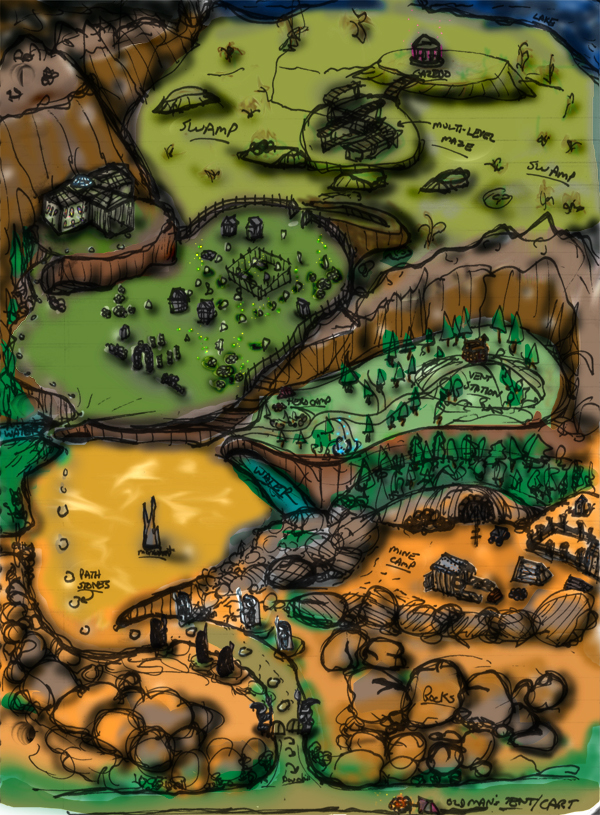
\includegraphics[width=200pt]{images/map_design.jpg}
	
\includegraphics[width=200pt]{images/aboriginal_art.jpg}
	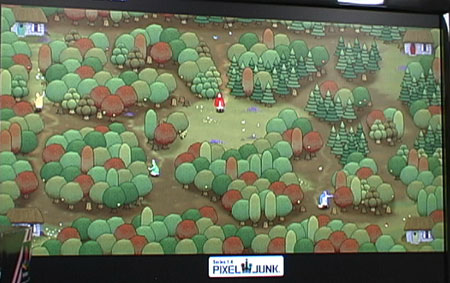
\includegraphics[width=200pt]{images/forest.jpg}
\end{center}
	\caption{impressions}\label{fig:global_map}
\end{figure}


\section{The problem: User control in procedural generation}

\desc{
Engineering theses tend to refer to a "problem" to be solved where other disciplines talk in terms of a "question" to be answered. In either case, this section has three main parts:
1. a concise statement of the question that your thesis tackles
2. justification, by direct reference to section 3, that your question is previously unanswered
3. discussion of why it is worthwhile to answer this question.
Item 2 above is where you analyze the information which you presented in Section 3. For example, maybe your problem is to "develop a Zylon algorithm capable of handling very large scale problems in reasonable time" (you would further describe what you mean by "large scale" and "reasonable time" in the problem statement). Now in your analysis of the state of the art you would show how each class of current approaches fails (i.e. can handle only small problems, or takes too much time). In the last part of this section you would explain why having a large-scale fast Zylon algorithm is useful; e.g., by describing applications where it can be used.
Since this is one of the sections that the readers are definitely looking for, highlight it by using the word "problem" or "question" in the title: e.g. "Research Question" or "Problem Statement", or maybe something more specific such as "The Large-Scale Zylon Algorithm Problem." 
}

\subsection{Rigidity of Procedural methods} 
\revise{bedenk een betere titel}

\subsection{User control} 

\todo{elke van de volgende controls behandelen met behulp van bestaande tools die hier gebruik van maken}
\begin{enumerate}
\item drawing techniques
\item modeling tools
\item parameters
\end{enumerate}


\subsubsection{local control}


\subsubsection{global control}


\subsection{Growing surfaces: An alternative method for area generation}


 

\section{Using realtime dynamically growing surfaces}

\subsection{dynamic structures: polygonal surfaces}
\inhoud{2D polygonale expansie van een ondergrond model als land of water die wordt gestuurd door eigenschappen van het type maar ook door ruimtelijke manipulatie methodes zoals vectorfields. representatie(onder voorbehoud): 
\begin{itemize}
\item Cellular automata
\item Cell systems
\item iets wat niet met cellen werkt  
\end{itemize}
realtime hertriangulatie zal moeten worden toegepast. 
polygonal meshes: 
\begin{itemize}
\item representation for irregular 2D volumes.  
\item suitable for water, land, cave like structures  
\item real-time demand, so need for efficient algorithms
\item houdt rekening met triangulatie
\item houdt rekening met smoothing
\item datastructure
\end{itemize}
citeer: On Vertex-Vertex Systems and Their Use in
Geometric and Biological Modelling
}

\todo{dit kan al snel worden geimplementeerd dus logisch om dit als eerste te beschrijven en methode uit te werken.}

\voegtoe{beschrijf waarom ik dynamic modeling technieken nodig heb}



\voegtoe{review methodes for dynamic modeling}


\voegtoe{focus op cell systems}


\voegtoe{custom systeem dat alle eigenschappen heeft die nodig zijn voor de polygonale expansie}



\cite{compgeom}
\cite{vertexsystems}

\subsection{l-systems and map l-system type spatial growth patterns}

\cite{lcreport}


\subsection{Real-Time spatial growth Models For Outdoor Areas}
\inhoud{Per type spatial growth model bespreken wat de context is binnen outdoor areas en dus met 
welke andere spatial growth modellen het communiceert en welke effecten het spatial growth model heeft 
op de andere en vica versa. Ook bespreken op wat voor manier een vector field (en andere tools 
die invloed hebben op de ruimtelijke indeling)  effect heeft op de uitdijing van dit type model.   
}

\subsubsection{Land} 
\todo{beschrijven hoe land expansie verloopt en hoe het communiceert met andere modellen}

A definition of land: "The part of Earth which is not covered by oceans or other bodies of water".(bron: http://en.wiktionary.org/wiki/land ...jaja ik vind nog wel een betere bron)
In reality land obviously does not grow, so first we must ask ourselves whether growing land in our virtual world can be made useful and intuitive to use. There are no real rules for the bounding shape of a piece of land, the bounds can be configured in any way. However due to this fact almost any random configuration of the shape of land looks realistic. The question is, as with other growth models with a minimum amount of rules, whether generating land by means of a growth model, thereby having less control over the result compared to conventional methods, is something which we want. 

When you want maximum control over the resulting geometry of a piece of land, using a growth model is not a very attractive method.However there are some situations in which this method is quite helpful.

\inhoud
{wanneer is het groeien van land handig: 
\begin{itemize}
\item Obviously: In situaties waarin de gebruiker niet veel waarde hecht aan de precieze vorm van de resulterence geometrie.  
\item stimuleert de creativiteit: elaborate. 
\end{itemize}
}

Land provides the underlying surface of many of the growth models discussed in this paper. 

\inhoud
{dus het bestaan van land op de seedpositie van een afhankelijk groeiproces is een eis. Wellicht moet het genereren van een map bestaan uit verschillende fases:
\begin{itemize}
\item fase 1: generatie van land en water. 
\item fase 2: plaatsen en activeren van groei processen die afhankelijk zijn van land.  
\end{itemize}
}

The field of biological modeling provides some interesting modeling techniques for the process of cell division. 
Cell division is interesting with respect to the concept of growing land because it is an expanding process with some nice properties. \voegtoe{benoem properties of revise deze zin.} 


\subsubsection{Water} 

\subsubsection{Roads}

\subsubsection{Afforestation} 

\subsection{Real-time spatial growth models For Indoor Areas}

\subsubsection{Caves}

\subsubsection{Canarian Aboriginal style homes}

\section{Organic map generation tool}

\subsection{Modifiers}

\subsubsection{Spatial modifiers}

\inhoud{
\begin{itemize}
\item vector fields: dit moet je wellicht helemaal aan het begin doen omdat alle spatial growth models
gemanipuleerd worden door deze vector fields.
\item obstruction with solid objects
\item smudge-like tool
\end{itemize}
}

\subsubsection{Timeflow modifiers}
\inhoud{
\begin{itemize}
\item pause model
\item speed up model
\item slow down model
\item reverse time flow
\end{itemize}
}


\subsection{User controlled map generation}

\subsection{automatic map generation} 


\section{Implementation}
\subsection{Tools used}
\inhoud{ 
\begin{itemize}
\item programming language: c++ (for now)
\item visualization library: openGL or Ogre3D (if it features easy vertex manipulation) 
\item physics engine: ODE (onder voorbehoud)  
\item collision detection: D-Collide (onder voorbehoud)
\end{itemize}
}

\subsection{Application Class Structure}

\voegtoe{
klassen structuur(voorlopig):
\begin{itemize}
\item Environment or Canvas: mainloop
\item Seedpoint  
\item GrowthModel 
\item ShapeModel
\item NetworkModel
\item ModelHistory
\item ModelTopology
\item ModelGeometry 
\item EventHandler
\item Communicator
\item Timeline: can place seeds on the timeline which will be handled by eventhandler when time comes.  
\end{itemize}
}






\subsection{User Interface}
\subsection{Communication system between models}

\section{Results}

\section{Conclusion}





%references
%logische volgorde:
%introduction: context-> previous work  
%method
%implementation
%results 
%conclusion 
\newpage 
\bibliographystyle{abbrv}	% (uses file "plain.bst")
\bibliography{thesisrefs}	% expects file "myrefs.bib"

\end{document}

